\documentclass[tikz,border=3.14mm]{standalone}
\begin{document}
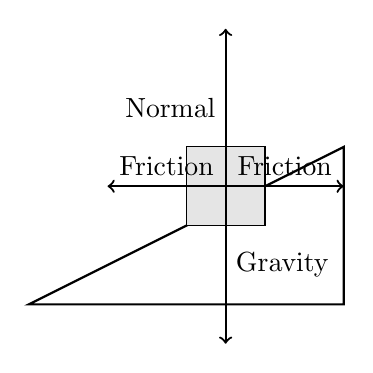
\begin{tikzpicture}
    % Draw the inclined plane
    \draw[thick] (0,0) -- (4,0) -- (4,2) -- cycle;

    % Draw the box
    \draw[fill=gray!20] (2,1) rectangle +(1,1);

    % Draw the forces
    \draw[thick,->] (2.5,1.5) -- +(0,-2)  node[midway,right] {Gravity};
    \draw[thick,->] (2.5,1.5) -- +(1.5,0) node[midway,above] {Friction};
    \draw[thick,->] (2.5,1.5) -- +(-1.5,0) node[midway,above] {Friction};
    \draw[thick,->] (2.5,1.5) -- +(0,2) node[midway,left] {Normal};
\end{tikzpicture}
\end{document}